\documentstyle[cec2003,multicol,times,epsfig]{article}

\begin{document}
\pagestyle{empty}
\sloppy

\twocolumn[
\title{SimME\\Mobile Multiplayer Gaming}

% list of authors with occupation
\vspace{2mm}
\begin{multicols}{4}
\begin{center}
	Wolfgang Slany\\
	\emph{Project Lead}\\
	wsi@ist.tugraz.at
\end{center}
\begin{center}
	Paul Sprenger\\
	\emph{Technical Documentation}\\
	sprenger@sbox.tugraz.at
\end{center}
\begin{center}
	Georg Spielmann\\
	\emph{User Interface}\\
	schurli@users.berlios.de
\end{center}
\begin{center}
	Kariem Hussein\\
	\emph{Architecture and Design}\\
	kariem@users.berlios.de
\end{center}
\end{multicols}
\vspace{0.25in}
] % end of the argument to \twocolumn

\begin{abstract}

	SimME is a multiplayer game for mobile devices (mobile phones, PDAs, ...)
	developed to provide a basis for a gaming forum in which new games can
	easily be integrated. The architecture described in this document is
	targeted on assisting the implementation of multiplayer games for mobile
	devices.

\end{abstract}


\section{Introduction}

	A lot of game developers, particulary developers working in the area of
	wireless communication, are confronted with the same problem: a two player
	game is usually limited to infrared or bluetooth communication, depending on
	the device capabilities. A server-based version for multiplayer gaming is
	unlikely, due to limited resources on mobile devices.

	On the basis of this consideration the SimME project tries to create a
	platform in which a server-based multiplayer version of an existing game can
	be created with minimal effort. The communication is based on internet
	technologies, a domain where most mobile device vendors focus their
	development.

	Because of the strict partitioning of game logic and communication between
	client and server, we have achieved that the server-side only has to
	implement the communication protocol between client and server. In fact, the
	server is only a mean of documented communication. Games could be viewed at
	a later point in time and player performance can be logged and compared.
	
	Figure \ref{fig:communication} shows how users can play SimME over the
	internet.
	
	\begin{figure*}[htbp]
		\begin{center}
			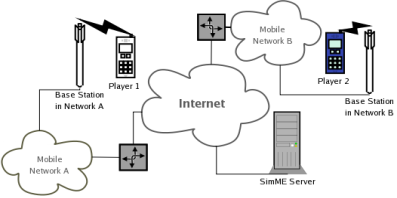
\includegraphics{pics/communication-small.png}
			\caption{Communication between clients on two different networks}
			\label{fig:communication}
		\end{center}
	\end{figure*}


\section{Applied Theory - Ramsey's Theorem}

	The game's rules build on Ramsey's theorem. Here is a short description
	\cite{wiki}:
	
	Ramsey's Theorem, named after the English mathematician Frank P. Ramsey,
	states that in colouring a large complete graph, one will find complete
	subgraphs all of the same colour. In a precise statement, for any pair of
	positive integers (r,s), there exists an integer R(r,s) such that for any
	complete graph on R(r,s) vertices, whose edges are coloured red or blue,
	there exists either a complete subgraph on r vertices which is entirely
	blue, or a complete subgraph on s vertices which is entirely red. Here
	R(r,s) signifies an integer that depends on both r and s. This initiated the
	combinatorial theory, now called Ramsey theory, that seeks regularity amid
	disorder
	
	\subsection{Ramsey Numbers}
	
		The numbers R(r,s) in Ramsey's theorem (and their extensions to more
		than two colours) are known as Ramsey numbers. An upper bound for R(r,s)
		can be extracted from the proof of the theorem, and other arguments give
		lower bounds. However, there is a vast gap between the tightest lower
		bounds and the tightest upper bounds. Consequently, there are very few
		numbers r and s for which we know the exact value of R(r,s).
		
		At the time of writing, even the exact value of R(5,5) is unknown,
		although it is known to lie between 43 and 49 (inclusive), and, barring
		a breakthrough in theory, it is probably the case that the exact value
		of R(6,6) will remain unknown forever.
	
		\begin{quotation}	
		
			Imagine an alien force, vastly more powerful than us landing on
			Earth and demanding the value of R(5, 5) or they will destroy our
			planet. In that case, we should marshal all our computers and all
			our mathematicians and attempt to find the value. But suppose,
			instead, that they asked for R(6, 6), we should attempt to destroy
			the aliens---\emph{Paul Erd\"os}
		
		\end{quotation}
		
	\subsection{Party Puzzle}
	
		This theory brings us to the Party Puzzle which consists in the question
		of how many people do you have to take, randomly chosen, on a party so
		that either 3 of them know each other mutually or 3 of them don?t know
		each other mutually. The answer to this question corresponds to the
		Ramsey number R(3,3) = 6.

		Let's name the 6 people A, B, C, D, E, F and G then we only have to
		consider 2 cases:
		
		\begin{itemize}
			
			\item In the first case, suppose A knows three (or more) of the
			others, say, B, C and D. If either B and C, B and D, or C and D are
			mutual acquaintances, then A and the acquainted pair make three
			people who know one another. Otherwise B, C and D are mutual
			strangers.
			
			\item In the second case, suppose A knows only two (or fewer) of the
			others, say, B and C. If either D and F, D and E, or E and F are
			strangers, then A and the unacquainted pair make three people who do
			not know one another. Otherwise D, E and F are mutual acquaintances.
			
		\end{itemize}
		
		This puzzle can be illustrated by our game SimME in which the 6 people
		are represented by 6 vertices. The relationship between two people --
		strangers or acquaintances -- is represented by colored edges between
		the corresponding vertices.


\section{Description of the Game}

	SimME describes the the party puzzle, a special case of the Ramsey theory.
	The game board consists of six points arranged at the corners of a hexagon.
	One point is connected to the other five points. At each turn, one player
	connects two points. The player who connects three points with a triangle
	loses the game.
	
	Figure \ref{fig:gameboard} shows an empty game board on the client device.
	As the game progresses, connections between points (edges) are marked with
	the player's colour.

	\begin{figure}[h]
	\begin{center}
		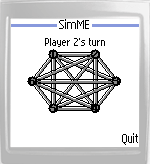
\includegraphics{pics/simme-screen.png}
		\caption{SimME game board on mobile phone}
		\label{fig:gameboard}
	\end{center}
	\end{figure}

	The game can never end in a draw, there is always a winner. Due to the
	odd number of connections between the vertices of the hexagon, there can
	never be a stalemate. A close analysis of this game and the underlying
	Ramsey theory was done in the paper \emph{Graph Ramsey games} by
	Wolfgang Slany \cite{slany_paper}.

	The game is designed for mobile phones and allows either to play against
	the computer, or against another human player over the web. Therefor the
	game has a client-server architecture. More on this in section
	\ref{sec:architecture}.


\section{Current State of Development}

	Until now the game SimME was implemented in the following versions:

	\begin{itemize}
		\item one player game (against a computer opponent)
		\item local multiplayer game (two players - one device)
		\item multiplayer game (with an external game server)
	\end{itemize}

	The main focus lied on the strict isolation of client and server, to design
	game logic and communication between client and server as modular as
	possible. This should ensure optimal extensibility and allow for simple
	development of future games.
	
	A close look on the architecture follows in section \ref{sec:architecture}.
	Let's first take a closer look at the items stated above.
	
	\begin{enumerate}
	
		\item \textit{one player game (against a computer opponent)}
		
			A computer opponent is implemented. As described in section
			\ref{sec:ci} at this time there is no \textit{intelligent} computer
			opponent integrated in the game SimME, but an opponent taking
			randomised turns.
			
			The portation of a learning computer opponent, implemented as a java
			applet Version of the game (called HEXI) from Wolfgang Slany, is
			planned \cite{slany_paper}.
			
		\item \textit{local multiplayer game (two players - one device)}
		
			In this Version of the game SimME two players play local against
			each other. They share one mobile device an take turns one after the
			other.
			
			A local multiplayer game version will be the starting point
			for implementing a server based version of other games in the
			future.
			
		\item \textit{multiplayer game (with an external game server)}
		
			This version of the game is uses the design described in section
			\ref{sec:architecture}. Two human players connect to a game server,
			using their mobile device. This server is responsible for
			match-making, as there are usually more than only two people
			connected.
			
			In the current implementation (limited by MIDP 1.0), all
			communication passes the server.
			
	\end{enumerate}
	
	With these three game layouts the porting of an existing game to the
	SimME-platform can be described.


\section{Going online} \label{sec:going_online}

	Starting from a local multiplayer game, it is easy to implement the
	communication between two clients using an external server. The task is to
	create an interface used by the server and the client to communicate with
	each other.
	
	\begin{figure}[h]
	\begin{center}
		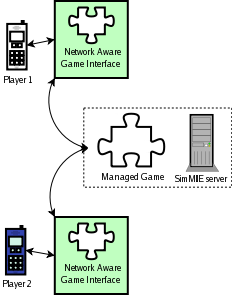
\includegraphics{pics/interface-usage.png}
		\caption{General game implementation: server manages a multiplayer game}
		\label{fig:interface}
	\end{center}
	\end{figure}

	How to build this interface? In a first step, the game's logic is
	abstracted. This abstract representation is used for single player games and
	multiplayer games on the client. The single player game extends the abstract
	game with simple AI logic, while a multiplayer game implementation that uses
	the intenet adds transparent network communication. The SimME server uses
	the general implementation and creates a \emph{managed game} for each
	multiplayer game. This is illustrated in figure \ref{fig:interface}.

	Whenever a move at player 1's mobile phone is performed, the managed game is
	updated accordingly. Player 2's mobile phone takes note of the updated game
	information, and updates its "local" game. In fact the game is transparently
	played at three locations, but the same implementation does not allow
	illegal or duplicate moves to be performed.

	
\section{Design and Architecture} \label{sec:architecture}

	As already said in section \ref{sec:going_online}, the game server can be
	seen as sole mediator between the game clients. The server has no access to
	the game logic, though it uses the client classes to verify correct
	gameplay, and to log the game as it progresses.
	
	With this approach, the game may be played between players on different
	continents, using the internet as mediation. Figure \ref{fig:communication}
	shows an example of two users, that use their mobile phones to connect to
	the internet, in order to play a game of SimME.
	
	\subsection{Advantages of the separation of server and game logic}

		Because of the separation of the game logic from the server, the server
		is nothing more than a link between the two players. All game internal
		check-ups are done by the clients and so the server is not charged.
		
		Further on its guaranteed that no \textit{needless information} is
		transferred. For example an illegal game turn is not transferred to the
		server, because the validation of moves is done in the clients. So the
		illegal turn will never arrive at the server or the second player.

	\subsection{Communication between client and server}

		The communication between client and server uses two different types of
		communication. On the one hand the client sends direct HTTP-requests, on
		the other hand the server answers with XML content. Figure
		\ref{fig:com_client_server} illustrates this.

		\begin{figure}[h]
		\begin{center}
			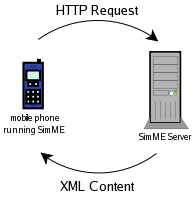
\includegraphics{pics/com_client_server.png}
			\caption{Communication between client and server}
			\label{fig:com_client_server}
		\end{center}
		\end{figure}

		The communication interface is backed by dynamic menus, created and
		administrated by the game server. These dynamic menus can be reused by
		other games because they are organised in interface-classes and
		consequently are modular. The layout and content is defined in XML and
		can be exchanged at run-time.

	\subsection{Internal administration on the server}
	
		The internal data organisation on the server side is carried out by
		means of a database, containing informations about the games currently
		running and about registered players. Further on with this database also
		the different games, implemented on the SimME-platform, will be
		administrated.
		
		Thus information about currently registered players, running games, and
		so on can be obtained via SQL statements.
		
		One of our next goals is to implement, alternatively to improve, the
		statistic part of the database. In this way statistics about gaming
		behaviour, win-lose statistics and much more can be implemented.


\section{Computational Intelligence} \label{sec:ci}

	At the current state of development there is no implementation of a CI
	gaming unit available on the SimME-server. The same game (also known under
	the name of HEXI) was realised as a java applet by Wolfgang Slany. In this
	version of the game, playable on
	\textit{http://www.dbai.tuwien.ac.at/proj/ramsey/} a learning computer
	opponent is implemented. You can take a closer look on the implementation of
	this CI gaming unit in \cite{slany_paper}
	
	\noindent Online version of this paper:\\
	http://www.dbai.tuwien.ac.at/ftp/papers/slany/dbai-tr-99-34.ps.gz

	\subsection{CI Player for SimME}
	
		The CI gaming unit mentioned above will be integrated in the single
		player version of the game SimME. On the client as on the server side.
		Through the implementation of the CI gaming unit on the SimME-server we
		get the possibility to record statistics about gaming strategies,
		because sole moves and therefor whole game matches could be logically
		analysed.
		
		Furtheron the learning CI gaming unit could even \textit{learn} from
		matches played by two human players.
		
		Based on these statistics an adjustment of gaming levels of the
		CI-gaming-unit could be done, so to each player a CI player with the
		same gaming level can be assigned.


\section{Look-out on future developments}

	In this section some ideas are listed we will implement in the future.
	
	\subsection{Player communication during a running game}
	
		Like Tony Manninnen says in "Interaction Forms and Communicative Actions
		in Multiplayer Games" \cite{mann03}:
		
		\begin{quotation}
		
			Rich interaction is achieved through direct manipulation of objects,
			multimodal input devices and the high number of degrees of freedom.
			However, this relatively technical definition covers only one
			portion of the concept. In addition to these, social, cultural and
			communicative aspects have a significant impact on interaction
			richness. \ldots
		
			\textit{Rich interaction does not necessarily require rich
			interfaces.}
			
		\end{quotation}
		
		The last sentence of this quotation describes our approach to useful
		communication forms between players really good. The idea is to provide
		some \emph{hardcoded} sentences which can be sent to the second player.
		In the first place its a very time saving way to communicate in written
		form - which is important because of the online costs of mobile devices.
		Secondly, with fixed sentences, a database can be used for translating
		these sentences to different languages at minimal costs.
		
		Of course it is also planned to implement a chat functionality to aid a
		free form of communication.
	
	\subsection{Integration of a CI gaming unit}

		As described in \ref{sec:ci} a CI gaming unit will be integrated in the
		SimME server and optionally on client side. It is possible that this
		unit uses too much space, which is a scarce resource on most mobile
		phones. This unit supports a challenging single player version one the
		one hand, and improves the value of game statistics on the other hand.
		
		The CI gaming unit implemented by Wolfgang Slany is a learning opponent,
		so the recorded games will be used by the CI gaming unit to improve the
		its performance.
	
	\subsection{Game statistics}

		A ranking system among users with sophisticated performance statistics
		will be implemented to raise user satisfaction. Besides win and loss
		counts these statistics will show the following data:
		
		\begin{itemize}
		
			\item Rating based on move effectiveness
			
			\item Number of moves to win a game
		
			\item Game length
			
			\item Move length, which denotes how fast the player executes a move.
		
		\end{itemize}


\section{Conclusion}

	The game itself is under development, and some additional features are being
	implemented at the time of this writing. We hope that we could give a
	thorough overview of SimME and the game's design.



\begin{thebibliography}{10}

	\bibitem[slany99]{slany_paper} Slany W. (1999) "Graph Ramsey games",
	Institut f\"ur Informationssysteme Abteilung Datenbanken und Artificial
	Intelligence Technische Universit\"at Wien
	
	\bibitem[mann03]{mann03} Manninen T. (2003) "Interaction Forms and
	Communicative Actions in Multiplayer Games", The international journal of
	computer game research
	
	\bibitem[wiki04]{wiki} Wikipedia.org (2004) "Ramsey's theorem", Wikipedia --
	The Free Encyclopedia: http://en.wikipedia.org/wiki/Ramsey's\_theorem
	
\end{thebibliography}

\end{document}
